\documentclass[english]{article}

\usepackage{graphicx}
\usepackage{grffile}
\usepackage{babel}
\usepackage{parskip}
\textwidth = 426pt
\oddsidemargin = 17pt

\author{
	Mufamadi, Khodani\\
	\texttt{14197520}
	\and
	Burgers, Heinrich\\
	\texttt{150595538}
	\and
	Cheriyan, Midhun\\
	\texttt{17308632}
	\and
	Cilliers, Joshua\\
	\texttt{14267196}
	\and
	Leshaba, Harris\\
	\texttt{15312144}
	\and
	Van Hattum, Jason\\
	\texttt{15027458}
	\and
	Rambani, Unarine\\
	\texttt{14004489}
}

\title{Cos301 : Software Requirements Specification\\
	for the NavUP System\\
	}
\date{\today}
\graphicspath{{Pictures/}}

\begin{document}
	\maketitle
	\begin{figure}[!t]
		
\includegraphics{up_logo.png}
	\end{figure}
	\pagenumbering{gobble}
	\newpage

	\tableofcontents
	\newpage

	\pagenumbering{arabic}
	

	\section{Introduction}
			

		\subsection{Purpose}
			The purpose of this document is to give a detailed description of the requirements for the NavUP System, it  will illustrate the purpose and complete declaration for the development of the system. It will also explain system constraints, interfaces and interactions with other external applications. This document is primarily intended to be proposed to a client for its approval, as well as the stakeholders and other interested parties. This document  will also serve as a reference for developing the first version of the system for the development team.

		\subsection{Scope}
			NavUP System is a WiFi-based mobile navigation application which helps users navigate to various venues, such as lecture halls, shops, restaurants and ablution facilities located on the University of Pretoria's Hatfield campus. Navigation is based on a user’s current location, accessibility needs and the pedestrian traffic information obtained from other users' locations. The application should be free to download from either a mobile phone application store or similar services.\\
			\\
			The system will make use of the university's WiFi infrastructure as well as the device's internet and GPS functionality to fetch and display results to users on their smart devices. The current location of the user should be determined both outdoors and indoors. Various activities that use location and movement of users can also be integrated.

		\subsection{Definition, Acronyms, and Abbreviations}
				This section of the SRS contains definitions, acronyms and abbreviations for the terminology used to describe our system throughout this document.
				\\
				\\
				\begin{tabular}{ |p{3cm}|p{9cm}|  }
				\hline
				\textbf{Term} & \textbf{Definition}\\
				\hline
				User & An actor that interacts with the mobile phone application \\
				\hline
				Administrator & An actor that is given specific permission for managing and controlling the system\\
				\hline
				\end{tabular}

		\subsection{References}
			[1] IEEE Software Engineering Standards Committee, "IEEE Std 830-1998, IEEE Recommended Practice for Software Requirements Specifications", October 20,1998

		\subsection{Overview}
				\begin{tabular}{ |p{3cm}||p{11cm}|  }
				\hline
				\multicolumn{2}{|c|}{This SRS document describes the NavUp system. It is divided into three major sections} \\
				\hline
				Section 1 & This section describes the document purpose and the project scope.This section also includes the definitions, abbreviations, and references used throughout this document \\
				\hline
				Section 2 & This section provides the product Persperctive and the product functions,And also describes the uses of NavUp and the user characteristics.The Constraints, assumptions and dependencies for NavUp are described in this section\\
				\hline
				Section 3 & This section describes the external interface requirements for the NavUp system and a list of functional requirements and performance requirements .Design constraints and software system attributes and as well as other requirements for the NavUp system are included in this section.\\
				\hline
				\end{tabular}
	\newpage
	\section{Overall Description}
		
		\subsection{Product Perspective}
			
				\subsubsection{System Interfaces}
				The mobile application will need to communicate to the GPS system service within the mobile device, which will in turn communicate with the physical GPS device to find the location of the user. The application will also make use of WiFi connectivity to triangulate the user's location, especially in situations where the user is indoors and the GPS is unreliable.
To enable the system to provide users with information regarding venues, points of interest, events and activities the mobile application will have to communicate with the database. The mobile application will only use the database to get, add and modify data.
				\begin{center}
										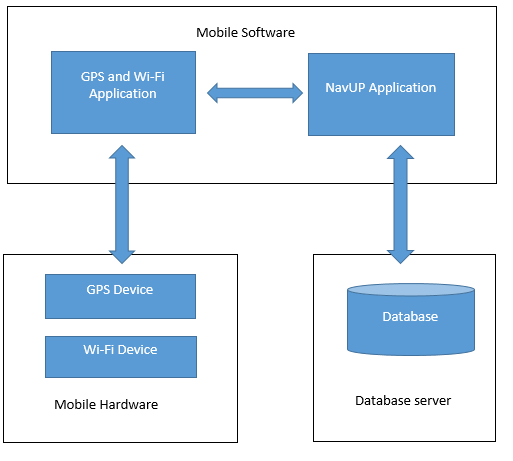
\includegraphics[scale=0.8]{Block Diagram.png}								
				\end{center}


				\subsubsection{User Interfaces}
						The system user interface must enable the user to perform basic navigation functions. Basic navigational functions required include searching for venues and providing directions to said venues. The system user interface should include functionality to visualise information related to pedestrian traffic on campus.

				\subsubsection{Hardware Interfaces}
				    Hardware interfaces that we shall make use of:
						\begin{itemize}
						    \item An android phone or tablet.
						    \item An iPhone or iPad.
						\end{itemize}

				\subsubsection{Software Interfaces}
				\begin{itemize}
					\item The mobile application will communicate with the GPS system service in order to obtain the geographical location of the user when the user is not inside a building.
					\item The mobile application will communicate with the university's router network to perform triangulation in order to find an approximate location of the user inside the building.
					\item The mobile application will communicate with the database to lookup events \& activities of interest and display them to the user to the user.
				\end{itemize}
						

				\subsubsection{Communications Interfaces}
				    Communications that we shall make use of:
					\begin{itemize}
					    \item Cellular networks
					    \item Global Positioning Satellites (GPS)
					    \item Wireless networking (WiFi)
					    \item E-mail
					\end{itemize}

				\subsubsection{Memory}
					The system must be memory efficient due to the fact that standard mobile devices do not have large amounts of memory and the application must be able to run simultaneously with other applications.  
                    Typical android and iOS devices have 1GB of RAM or more, therefore to prevent overloading the operating system the application must use at most 150MB of RAM while the application is running.
                    The application must not use more than 50MB of hard disk drive space.

		\subsection{Product Functions}
            Users will be able to use their handheld devices to navigate around the campus if they having trouble to find venues. The system will assist the user to avoid pedestrian traffic and find the quickest route to their desired venue. The system will be able to locate the user’s current location either inside or outside the building by the use of the Wi-Fi access points. The system will store different types of information such as social events and activities, venues using multiple types of devices and services.The different types of information will be store on database. 

		\subsection{User Characteristics}
				NavUP should have three user groups: A Students/Staff Member, Administrators, and a Guests.
				\subparagraph{Students and staff members}
    				\begin{itemize}
    					\item Students and staff members are registered and have numbers that can be used to identify them.
    					\item Students are likely to be young (Below the age of 30).
    					\item Students and staff members are likely to have a high level of education.
    					\item Students and staff members should have a relatively high level of technical experience, and therefore be able to use and navigate a relatively complex app.
    				\end{itemize}
				\subparagraph{Guest Users}
    				\begin{itemize}
    					\item Guests are unregistered.
    					\item The technical level and education of a guest is unknown. 
    					\item It might be difficult for them to navigate a complicated interface.
    
    				\end{itemize}
				\subparagraph{Administrators}
    				\begin{itemize}
    					\item Administrators should have a high level of technical expertise.
    					\item Administrators likely have some form of identification, such as staff numbers.
    				\end{itemize}
		\subsection{Constraints}
                The constraints that we must work around are:
			    \begin{itemize}
			        \item \textbf{Cost} - We do not have the funds to pay for expensive libraries and tools.
			        \item \textbf{Time} - We only have some part of a semester semester to design and implement this system. Another thing to consider is that our work force is comprised of third year and Honours students who are have to divide their time and attention to different modules , which is restrictive in terms of the actual work time for the project.
			        \item \textbf{Skills} - Our skills are varied, but mostly undeveloped, which may limit the utility of our solution.
			        \item \textbf{Scope} - Our scope is defined as a navigation system for the University of Pretoria, and so our solution will be limited as such.
			    \end{itemize}

		\subsection{Assumptions and Dependencies}
		\subsubsection{Assumptions}
	\begin{itemize}
		\item The application is free for all users.
		\item Users will access the application through hand-held devices.
		\item The system will be available 24/7.
		\item The system will be simple.
		\item The system can locate a user inside and outside the building.
		\item The system can detect pedestrian traffic around the campus.
		\item User friendly system.
		\item Users are technically competent.
		\item The system and its user will have access to the university's Wi-Fi infrastructure.
		\item Users operating system is either Android or IOS.
		\item Users will be willing to provide personal information.

\end{itemize}


\begin{large}
	\subsubsection{Dependencies}
	\end{large}
	\begin{itemize}
		\item Teams' time and abilities. 
		\item Feedback from stakeholders. 
		\item A database to store social activities and different venues.
		\item The application needs access to WiFi.
		\item Adequate advertisement. 

	\end{itemize}
	\newpage

	\section{Specific Requirements}
				\subsection{External Interface Requirements}
					    Since the prototype will most likely only be developed for Android systems and later expanded to iOS and other systems, this part of the specification will primarily assume the Android OS is the operating system for the system.
					    \subsubsection{Interfaces} 
					     The app will require system privileges to make use of certain features and information provided by the Android OS.
					    \begin{itemize}
					        \item  \textbf{Communication Protocols}\\
					        The system will be dependant on making use of the connection to the Internet provided through the device's connection to WiFi or mobile data. This will be necessary for the main functions such as mapping, location tracking, navigation and heatmaps (for traffic avoidance) to work.
					        \item \textbf{GPS}\\
					        The system will be dependant on the device's GPS system services to be able to accurately track both where the users are and where they are going. Access to this feature forms the backbone of the app as nearly all our subsystems are dependant on it.
					    \end{itemize}

					    \subsubsection{User Interfaces}
					     There will be a unified user interface which can be broken down into 5 subsystems all of which will be displayed simultaneously. The 6th subsystem (Suggestive Searching) will tie into the navigational subsystem.\\
					    \begin{itemize}
					        \item \textbf{Navigation}\\
					        Users will use the navigation subsystem to select a new destination, as well as deciding on their starting point. This information will be sent through to the mapping and location subsystems. It will eventually receive output from the mapping subsystem in the form of a route to follow which it will forward on to the display subsystem to display on screen for users.
					        \item \textbf{Location}\\
					        Users will passively interact with the location subsystem as it will autonomously track the device's location for input which the Navigation, Mapping, and Heatmap subsystems will use. It will continuously update the device's location and provide it as output to the mapping and/or navigational subsystem depending on context.
					        \item \textbf{Mapping}\\
					        This will calculate the route which the user has to take. It will accept input from the Location, Heatmaps, and the Navigation subsystems and then use that information to calculate the best possible route which it will provide as output.
					        \item \textbf{Heatmaps}\\
					        This will make use of information provided by the university's network to discover how many people are connected to routers in certain areas at particular times. It will compare this to it's own averages gathered over time to calculate whether or not an alternative route or warning should be displayed due to high amounts of pedestrian traffic in certain parts of campus.
					        \item \textbf{Games and Events}\\
					        These events and games will be managed by administrators who are given more privileges. It's suggested that a form of validation and moderation is placed either on the people given these privileges or on the events and games that they wish to add to the system. These games and events will then be added into the map so that they can be displayed and interacted with by the users.
					        \item \textbf{Suggestive Searching}\\
					        This will be a minor add-on to the Navigational Subsystem which will suggest new locations and events to users based on their existing searches.	        
					        
					    \end{itemize}
    					\subsubsection{Interfaces}
    						\begin{itemize}
    						    \item \textbf{An android phone or tablet} \\
    						    Android devices are the most commonly used devices, so development will initially focus on these devices. There are android devices with many varying specifications, but we will focus on newer models in order to simplify the prototype. \\
    						    \item \textbf{An iPhone or iPad} \\
    						    iOS devices are not focused on initially due to the face that only a small percentage of staff and students use iPhones or iPads.
    						\end{itemize}
    						
    					\subsubsection{Software Interfaces}
        					\begin{itemize}
        					    \item \textbf{Google Maps API}\\
        					    This would be our tool of choice as it covers the basis for navigation and mapping subsystems, which NavUp requires for successful implementation.
        					    \item \textbf{Other}\\
        					    Other libraries and API's will then be added to the project later to cater for any extensions once our core features have been implemented.
        					\end{itemize}

						\subsubsection{Interfaces}
    						\begin{itemize}
    						    \item \textbf{Cellular networks} \\
    						    We will use cellular networks in conjunction with WiFi to transmit data such as user credentials, heatmaps, and routing which required to use the app. \\
    						    
    						    \item \textbf{Global Positioning Satellites (GPS)} \\
    						    We will make use GPS to locate the device for heat-map generation and navigation.    						    
    						    \item \textbf{Wireless networking (WiFi)} \\
	    						    WiFi will be used to locate the device similar to GPS, especially inside where GPS connection may be poor. WiFi will also be used where possible to download and upload data similar to cellular networks. 
    						    \item \textbf{E-mail} \\
    						    We will use email for registration and login, which will then allow us to identify different users.  \\
    						\end{itemize}
    						
				\subsection{Functional Requirements}
					\begin{itemize}
					    \item \textbf{Requirement 1 (R1)}\\ The system shall allow users to create a profile to log in and out of, or it should make another allowance for their personal data to be associated with them. This data could alternatively just be stored locally on their device, similarly to a cookie for a website. The personal data is needed to store users personal searches which are needed for the Suggestions subsystem. Once the users have entered their details a request is sent to the server and they will be logged in to the system if their details were correct. If they aren't then an error will be generated declaring that their details were incorrect. \textbf{Priority : Important but not vital}
					    \item \textbf{Requirement 2 (R2)}\\ Regardless of the task that a user is performing, the system shall always generate an error if the device has no connection to the Internet. The error will be dismissable but until a connection to the Internet is restored, the system shall only have access to partial functionality. \textbf{Priority : Critical}
					    \item \textbf{Requirement 3 (R3)}\\ The system shall provide users with the ability to select a starting location. Users can either have the app automatically detect their location or they can manually enter a location of their choice. The Location Subsystem will have to perform a validity check on manual addresses to check that they are real. If they aren't an error will be generated declaring that the address couldn't be found. \textbf{Priority : Critical}
					    \item \textbf{Requirement 4 (R4)}\\ The system shall provide users with the ability to select a destination. Users will have to manually enter a destination. The Location Subsystem will have to perform a validity check on the address to check that they are real.  If they aren't an error will be generated declaring that the address couldn't be found.  \textbf{Priority : Critical}
					    \item \textbf{Requirement 5 (R5)}\\ The system shall provide users with the ability to request a route between the starting location and destination. The system will send both points to the Mapping Subsystem after they have been validated by the Location Subsystem. The mapping system will then calculate the optimal route between the two points. This route will be displayed as output to the user. If no route is available then the system will generate an error describing so. \textbf{Priority : Critical}
					    \item \textbf{Requirement 6 (R6)}\\ The system shall create an alert for users for if the heatmaps subsystem detects there is high traffic on the shortest route or if there are other hazards on campus. The values tallied by the Heatmaps Subsystem will have to compare the real-time values to recorded averages to decide whether there is actually traffic or not. If the Heatmaps Subsytem can't receive any data from the system it should generate an error describing that the traffic feature is offline. \textbf{Priority : Important but not vital}
					    \item \textbf{Requirement 7 (R7)}\\ The system shall also provide the option of calculating a detour in the previous scenario if the user wants. This links back to the Mapping Subsystem which can use an intermediary location to create a detour between the two points. \textbf{Priority : Important but not vital}
					    \item \textbf{Requirement 8 (R8)}\\ The system shall suggest new locations on campus to users based on their searches. These searches will be tied to their profile and the suggestions will be built off of that. This system should generate an error if the file containing user's searches can't be accessed. \textbf{Priority : Nice to have, not vital}
					    \item \textbf{Requirement 9 (R9)}\\ The system shall allow 'content creation' users to create events and games for other users to interact with. Additionally it will also allow lecturers to create a venue for lectures, tutorials or practicals in the case of unforeseen circumstances making it that normal arrangements don't hold. In the scenario that events can't be created or events and games can no longer be accessed, the system shall generate an appropriate error. 
					    \textbf{Priority : Nice to have, not vital}
					    \item \textbf{Requirement 10 (R10)} \\ The system shall allow users to interact with the events and games created by content creation users. If these events can't be accessed the system will generate
					    an error.
					\end{itemize}
				    \subparagraph{Use Case Diagrams}
				       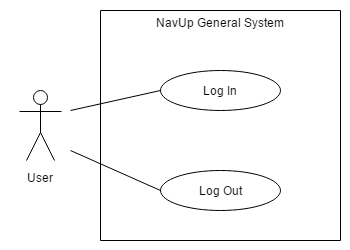
\includegraphics{NavUp_General.png}
				       \makebox[\textwidth]{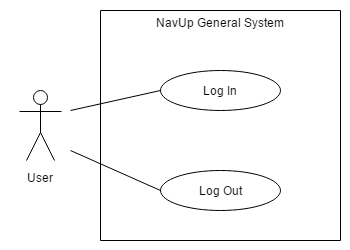
\includegraphics[width=\paperwidth]{NavUp_General.png}}
					   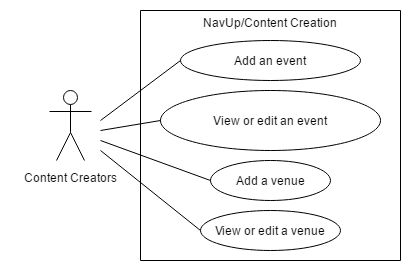
\includegraphics{NavUp_Content_Creation.png}
					   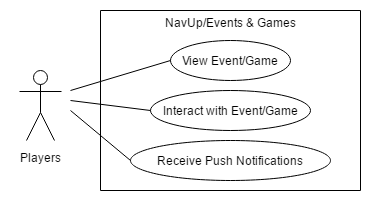
\includegraphics{NavUp_Events_and_Games.png}
					   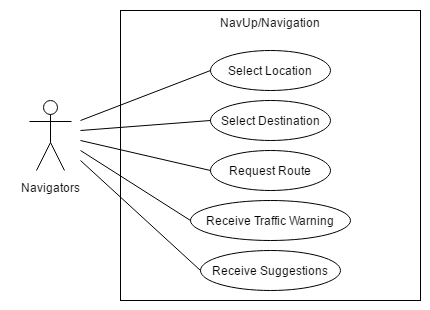
\includegraphics{NavUp_Navigation.png}		   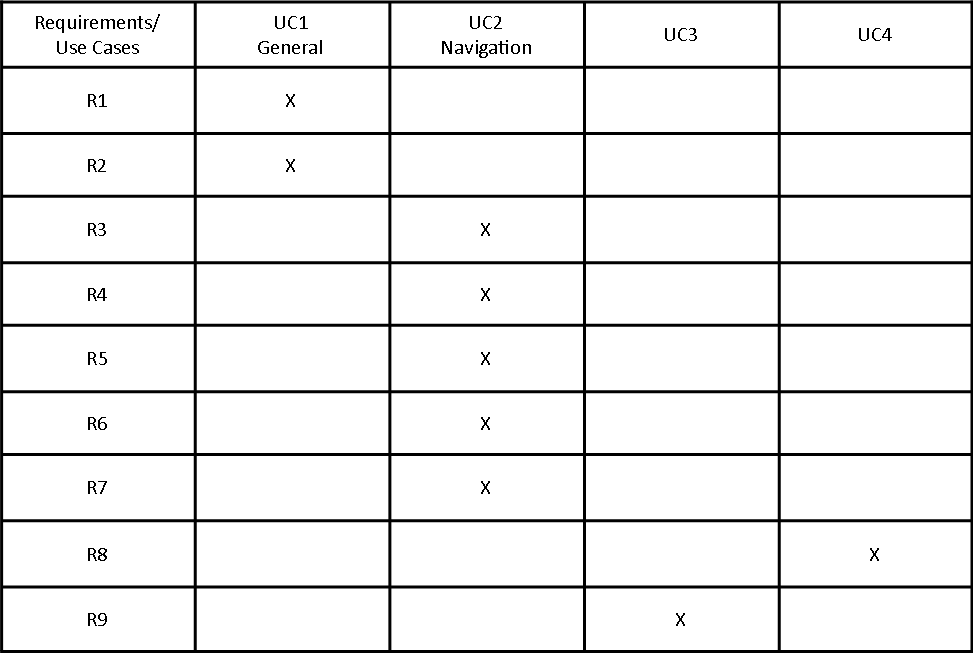
\includegraphics{Traceability_Matrix.png}

				\subsection{Performance Requirements}
    				The system must:
    				\begin{itemize}
        				\item Be interactive to user input within 2 seconds.
        				\item Acquire the user's location with an accuracy within an 8m radius.
        				\item Display the user's location on a map within 3 seconds after launching.
        				\item Generate routes for users within 2 seconds.
        				\item Update the user's location every second when navigating.
        				\item Give a warning or indication if the processes take longer than anticipated.
        				\item Display a message if an error is encountered.
    				\end{itemize}


				\subsection{Design Constraints}
				\paragraph\indent
				This application is constrained in two main areas, namely hardware and software. We will look at these two areas separately.
				 \subparagraph{Hardware:}
					\begin{enumerate}
						 \item
						Application is constrained to the device’s ability to connect to the internet. 
						 \item
						The effectiveness of the device is constrained to its ability to communicate with the WI-FI network on campus.	
						 \item
						The application is also constrained to the device’s ability to display the map and navigation system. 
						 \item
						The ability of the device to run the application is also limited to the hardware available. 
						 \item
						The speed the application can perform at is constrained by the processing power and available memory of the devise.
					\end{enumerate}
				 \subparagraph{Hardware:}
					\begin{enumerate}
					\item
					The device must be able to locate its position to an accuracy of 3m. 
					\end{enumerate}
					 \subparagraph{Other:}
					\begin{enumerate}
					\item
					This system’s ability to give updates and events is constrained to external management and maintenance. (An administrator)   
					\item
					The application is constrained to the University of Pretoria’s campuses.
					\end{enumerate}
				\subsection{Software System attributes}
					\paragraph\indent
				
				\subparagraph{Reliability}
    				The system must be able to all its functions under the stated conditions and produce correct and consistent results. 
    				
    			\subparagraph{Portability}
    				\begin{itemize}
        				\item The system must be able to run on different operating environments or platforms i.e. the system must be able to run on iOS and android.
        				\item The system must be able to run on different mobile devices such as smartphones and tablets.
    				\end{itemize}
    				
    			\subparagraph{Robustness}
    				The system must be able to perform its required functions under rough or exceptional conditions. Since the system heavily depend on newtwork connections, however the application must be able to perform basic navigation functions offline.
    				
				\subparagraph{Security}
    				\begin{itemize}
        				\item Only administrators must be able to add data to the system.
        				\item The location of the user must not be broadcasted or used by another application. 
        				\item All data transmitted between subsystems must be encrypted.
    				\end{itemize}
    				
				\subparagraph{Reusability}
				    The system must be reusable, it must permit itself to be used in a similar or different context with or without extension or customization.
				    
				\subparagraph{Efficiency}
				    The system must be able to perfor m its functions and produce desired results with minimum expenditure of time and resources.
				    
				\subparagraph{Availability}
				    The system must be always available provided that the minimum hardware requirements are met
    				    
				\subparagraph{Accuracy}
    				\begin{itemize}
							\item
							The application must be accurate up to 3m to function indoors but can be less accurate outdoors.
							\item
							The heat maps can combine known statistics as well as live feed to be more accurate. 
						\end{itemize}
						
				\subparagraph{Adaptability}
					\begin{itemize}
							\item
							This application must be able to adapt to:
							  \begin{itemize}
								\item
								A change in heat map patterns, events like strikes, and a change in router locations.
								\item
								A loss of signal.
							\end{itemize}
						\end{itemize}
						
				\subparagraph{Manageability}
					\begin{itemize}
							\item
							It is vitally important for this application to have an interface for a managing team.
							\item
							Departments need to update events. 
							\item
							New locations need to be added.
						\end{itemize}
						
				\subparagraph{Interoperability}
					\begin{itemize}
							\item
							The application must function on Android as well as IOS.
						\end{itemize}
				
				\subsection{Other Requirements}
					\paragraph\indent
						\begin{enumerate}
						 \item
						The Application needs to be able to learn the habits of the user and guide him/her accordingly. 
						 \item
						The application needs to support custom destinations and needs to be able to store these destinations for later use.
						 \item
						The application must still be able to give possible routes in the absence of Internet connection.
						 \item
						The application must be able to determine a route from one point to another, even if the neither of the points are the user’s position.
					\end{enumerate}		
\end{document}
